\documentclass[tikz,border=3pt]{standalone}
\usepackage[utf8]{inputenc}
\usepackage[T1]{fontenc}
\usepackage{lmodern}
\renewcommand{\familydefault}{\sfdefault}
\usepackage{sansmath}\sansmath
\usepackage{chemfig}
\usepackage{pgfplots}\pgfplotsset{compat=1.18,/pgf/number format/use comma,/pgf/number format/1000 sep={.}}
\usetikzlibrary{arrows.meta,calc,positioning,decorations.pathmorphing,patterns}
% paleta del sitio
\definecolor{nar}{HTML}{E8680C}\definecolor{narc}{HTML}{FFB35C}\definecolor{hielo}{HTML}{FFF3E8}
\definecolor{tinta}{HTML}{1D1D1F}\definecolor{gris}{HTML}{6E6E73}\definecolor{lila}{HTML}{7C5CF0}
\definecolor{azul}{HTML}{2F6FD6}\definecolor{menta}{HTML}{17A673}\definecolor{coral}{HTML}{E8342A}
\begin{document}
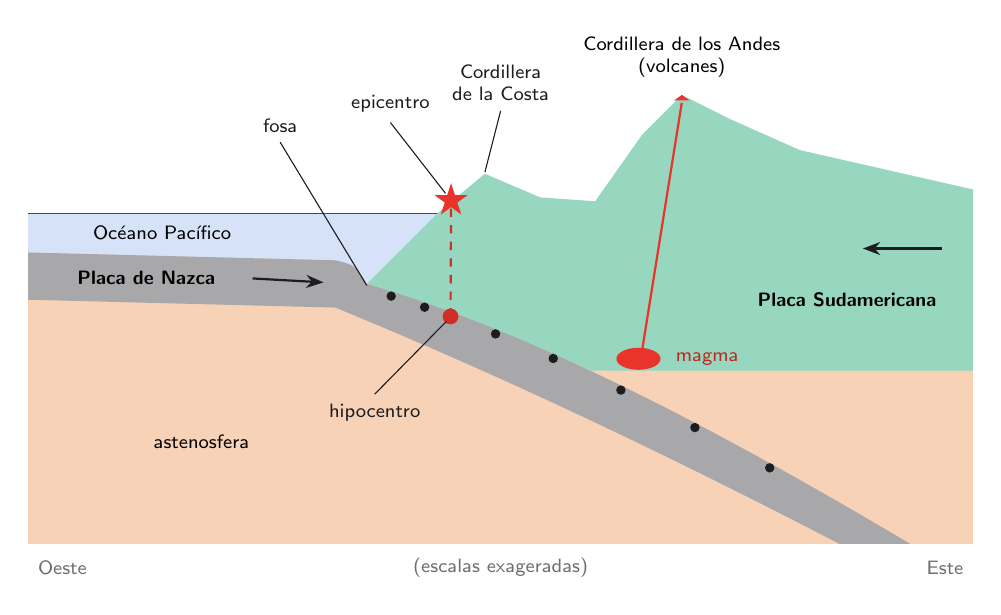
\begin{tikzpicture}[font=\footnotesize,>={Stealth[length=2.2mm]}]
% astenosfera
\fill[nar!30] (0,-4.2) rectangle (12,-0.5);
% agua
\fill[azul!20] (0,0) -- (5.2,0) -- (4.3,-0.9) -- (3.9,-0.6) -- (0,-0.5) -- cycle;
\draw[azul!70!black] (0,0) -- (5.2,0);
% placa sudamericana
\fill[menta!45] (4.3,-0.9) -- (5.2,0) -- (5.8,0.5) -- (6.5,0.2) -- (7.2,0.15) -- (7.8,1.0) -- (8.3,1.5) -- (8.9,1.2) -- (9.8,0.8) -- (12,0.3) -- (12,-2.0) -- (7.15,-2.0) -- (6.54,-1.73) -- (5.37,-1.25) -- cycle;
% placa de Nazca (subducta)
\fill[gris!60] (0,-0.5) -- (3.9,-0.6) .. controls (4.15,-0.66) .. (4.3,-0.9) .. controls (6,-1.4) and (8,-2.3) .. (11.2,-4.2) -- (10.3,-4.2) .. controls (7.6,-2.8) and (5.6,-1.9) .. (3.9,-1.2) -- (0,-1.1) -- cycle;
% volcan y magma
\fill[coral] (8.2,1.43) -- (8.4,1.43) -- (8.3,1.5) -- cycle;
\fill[coral] (7.75,-1.85) ellipse (0.28 and 0.14);
\draw[coral,thick] (7.8,-1.72) -- (8.3,1.4);
% hipocentros
\path (4.3,-0.9) .. controls (6,-1.4) and (8,-2.3) .. (11.2,-4.2)
  coordinate[pos=0.06] (h1) coordinate[pos=0.14] (h2) coordinate[pos=0.2] (h3) coordinate[pos=0.3] (h4)
  coordinate[pos=0.42] (h5) coordinate[pos=0.55] (h6) coordinate[pos=0.68] (h7) coordinate[pos=0.8] (h8);
\foreach \h in {h1,h2,h4,h5,h6,h7,h8} \fill[tinta] ($(\h)+(0,-0.06)$) circle (0.06);
\fill[coral!90!black] ($(h3)+(0,-0.06)$) circle (0.1);
\draw[coral!90!black,dashed,thick] ($(h3)+(0,-0.06)$) -- (5.37,0.14);
\fill[coral] (5.37,0.16) +(90:0.22) -- +(234:0.22) -- +(18:0.22) -- +(162:0.22) -- +(306:0.22) -- cycle;
\draw[tinta] (5.3,0.25) -- (4.6,1.15) node[above,font=\scriptsize] {epicentro};
\draw[tinta] ($(h3)+(-0.05,-0.12)$) -- (4.4,-2.3) node[below,font=\scriptsize] {hipocentro};
% rotulos
\node[font=\scriptsize] at (1.7,-0.25) {Océano Pacífico};
\node[font=\scriptsize\bfseries] at (1.5,-0.82) {Placa de Nazca};
\draw[->,thick,tinta] (2.85,-0.83) -- (3.75,-0.88);
\node[font=\scriptsize\bfseries] at (10.4,-1.1) {Placa Sudamericana};
\draw[->,thick,tinta] (11.6,-0.45) -- (10.6,-0.45);
\node[font=\scriptsize] at (2.2,-2.9) {astenosfera};
\draw[tinta] (4.3,-0.92) -- (3.2,0.9) node[above,font=\scriptsize] {fosa};
\draw[tinta] (5.8,0.52) -- (6.0,1.3) node[above,font=\scriptsize,align=center] {Cordillera\\de la Costa};
\node[font=\scriptsize,align=center,anchor=south] at (8.3,1.6) {Cordillera de los Andes\\(volcanes)};
\node[font=\scriptsize,text=coral!80!black,anchor=west] at (8.1,-1.85) {magma};
\node[font=\scriptsize,text=gris,anchor=west] at (0,-4.5) {Oeste};
\node[font=\scriptsize,text=gris,anchor=east] at (12,-4.5) {Este};
\node[font=\scriptsize,text=gris] at (6,-4.5) {(escalas exageradas)};
\end{tikzpicture}
\end{document}
